\item \textbf{{[}RVHS/PRELIM/9569/2021/P1/Q7{]} }

A relational database is created to store data about contractors engaging
workers to perform renovation jobs. 

The database designers are told that: 
\begin{itemize}
\item each contractor can recruit different workers to perform various jobs.
\item each worker can have skills to perform different jobs. 
\item each job can have different levels of skills \textquotedbl A\textquotedbl ,
\textquotedbl B\textquotedbl{} or \textquotedbl C\textquotedbl{}
and their hourly rate is calculated based on their skill level for
the job. 
\end{itemize}
A first attempt is represented by the following table: 
\begin{center}
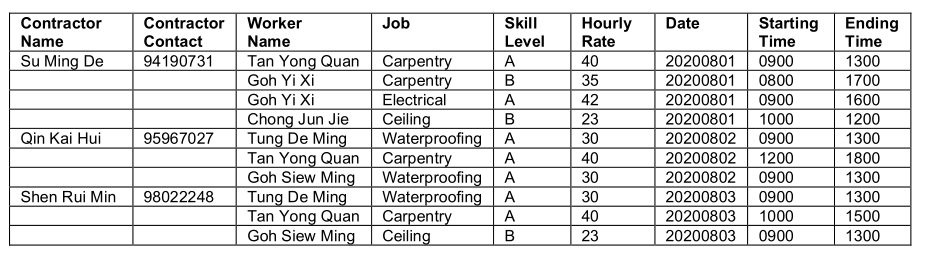
\includegraphics[width=0.65\paperwidth]{C:/Users/Admin/Desktop/Github/question_bank/LyX/static/img/9569-RVHS-2021-P1-Q7-1}
\par\end{center}
\begin{enumerate}
\item Explain why this table is not in first normalized form. \hfill{}{[}2{]}
\end{enumerate}
The following is an attempt to reduce data redundancy: 
\begin{center}
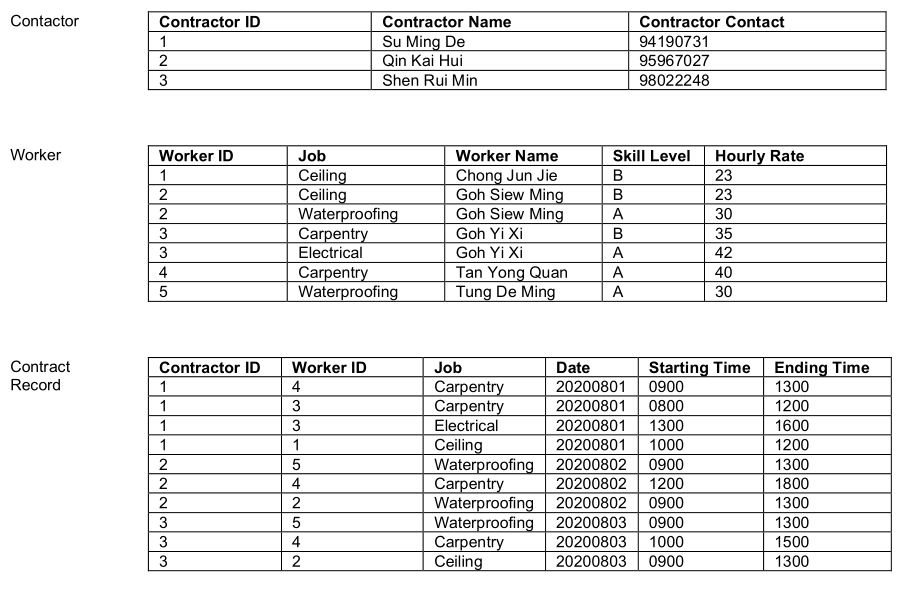
\includegraphics[width=0.65\paperwidth]{C:/Users/Admin/Desktop/Github/question_bank/LyX/static/img/9569-RVHS-2021-P1-Q7-2}
\par\end{center}
\begin{enumerate}
\item[(b)] Explain what a composite key is. \hfill{}{[}1{]}
\item[(c)] State a suitable primary key for Worker table and explain why the
table is not in second normal form. \hfill{}{[}3{]}
\item[(d)] A table description can be expressed as: 

\texttt{TableName (}\texttt{\uline{Attribute1}}\texttt{, Attribute2{*},
Attribute3, \dots ) }

The primary keys are indicated using a solid underline and foreign
keys are indicated by using a dashed underline/asterisk. Write table
descriptions for the required tables in the database so that they
are in third normal form (3NF). \hfill{} {[}6{]}
\item[(d)] Create an entity-relationship (ER) diagram showing the degree of
all relations. \hfill{}{[}3{]}
\item[(e)] Using the above example, elaborate why a relational database model
has advantage in maintaining data integrity over a flat file system.
\hfill{}{[}3{]}
\item[(f)] The homeowner would like to know a schedule of the renovation jobs
performed to their house. They are \textbf{NOT} interested in knowing
the exact worker\textquoteright s name. Write an SQL query to output
the \textbf{contractor\textquoteright s name}, \textbf{worker\textquoteright s
job}, \textbf{worker\textquoteright s skill level} and \textbf{date}
based on the contractor\textquoteright s name \textquotedbl\texttt{Su
Ming De}\textquotedbl . The output is to be in the ascending order
based on the date of job performed. \hfill{}{[}5{]}
\end{enumerate}